\section{Background and Motivation}\label{sec:background}

\subsection{Urban drone decisions are coupled}\label{sec:bg:coupled}

A city operator who dispatches a fleet of small multirotors for inspection, search or delivery repeatedly takes three
decisions for every sortie (Fig.~\ref{fig:scene}).
\emph{Launch precheck}: can this drone reach the task, stay on station and come back with the required energy reserve,
and is the wind along its route within the vehicle's rating?
\emph{Return planning}: when the battery or the operator calls the drone home, at which altitude and along which path
does it fly, and when must the return start so that it still lands with a reserve?
\emph{Scan planning}: at which height and strip spacing must the fleet fly so that the camera resolves the targets
under the current visibility, and how many drones does that take?

Each of these decisions depends on several physical factors at once. The return altitude depends on the buildings
along the return line; the return trigger depends on the energy needed to fly that path against the wind; the scan
height depends on the visibility, which in turn changes the number of strips, the flight time per sortie and thus the
number of drones. A decision that sees only one factor is not merely less accurate: it is wrong in a systematic,
weather- and city-dependent way. Today the factors live in separate tools. Flight stacks such as
PX4~\cite{meier2015px4} return at a fixed altitude above the take-off point; drone simulators model one
vehicle's dynamics in a uniform wind~\cite{shah2017airsim,koenig2004gazebo}; city digital
twins~\cite{batty2018digitaltwins,ketzler2020digitaltwins,shahat2021citydigitaltwin} and Web 3D viewers~\cite{ogc2023_3dtiles,schuetz2020octree}
display geometry but do not simulate. We call a decision \emph{coupled} when it is computed from one consistent model of
city geometry, a time-varying weather field and vehicle energy, the same model that drives the simulated ground truth
and the operator's display.

\begin{figure}[t]
\centering
\resizebox{\textwidth}{!}{\begin{tikzpicture}[x=0.92cm,y=0.92cm,font=\scriptsize,
  bld/.style={fill=g4,draw=g2,line width=0.3pt},
  lab/.style={align=left,text=ink,font=\scriptsize,fill=white,fill opacity=0.85,text opacity=1,inner sep=1pt},
  num/.style={circle,fill=oursred,text=white,inner sep=0.8pt,font=\scriptsize\bfseries}]
  % ground
  \fill[g5] (-0.3,0) rectangle (12.6,-0.12);
  \draw[g2,line width=0.4pt] (-0.3,0) -- (12.6,0);
  % buildings
  \foreach \x/\w/\h in {1.85/0.45/1.2, 2.5/0.35/0.8, 3.0/0.7/2.9, 3.9/0.45/1.6, 4.6/0.6/2.2, 5.5/0.35/0.9,
                        6.2/0.55/1.4, 7.6/0.5/1.0, 8.3/0.4/1.8, 9.0/0.6/0.7}
    \draw[bld] (\x,0) rectangle ++(\w,\h);
  % home pad
  \fill[g1] (0.2,0) rectangle (0.8,0.06);
  \node[below=1pt,lab] at (0.5,0) {home};
  % fog layer over the scan area
  \fill[g3,opacity=0.25] (9.8,0) rectangle (12.5,1.7);
  \node[lab,fill=none,text=g1,anchor=east] at (12.5,0.4) {fog, MOR 200\,m};
  % targets
  \foreach \x in {10.2,10.9,11.6,12.2} \fill[ink] (\x,0) rectangle ++(0.05,0.12);
  % wind arrows, above everything
  \foreach \y/\l in {3.75/0.9, 4.1/1.15, 4.45/1.4}
    \draw[-{Stealth[length=3pt]},g2,line width=0.5pt] (7.4,\y) -- ++(-\l,0);
  \node[lab,fill=none,text=g2,anchor=west] at (7.5,4.1) {wind $\mathbf{w}(x,y,z,t)$, stronger aloft};
  % fixed-altitude return (crosses buildings)
  \draw[g1,dashed,line width=0.6pt,-{Stealth[length=3pt]}] (10.0,1.2) -- (3.75,1.2);
  \draw[g1,line width=0.5pt] (3.58,1.08) -- (3.82,1.32) (3.58,1.32) -- (3.82,1.08);
  \node[lab,text=g1,anchor=south] at (7.0,1.24) {fixed-altitude return};
  % geometry-aware return
  \draw[oursred,line width=0.9pt,-{Stealth[length=3.5pt]}] (10.0,1.2) -- (10.0,3.15) -- (0.5,3.15) -- (0.5,0.1);
  \node[lab,text=oursred,anchor=south] at (5.2,3.18) {return above the highest roof on its line};
  % drone
  \fill[ink] (9.85,1.15) rectangle (10.15,1.25);
  \draw[ink,line width=0.4pt] (9.8,1.29) -- (10.2,1.29);
  % scan heights
  \draw[g1,dotted,line width=0.7pt] (9.8,2.4) -- (12.5,2.4);
  \node[lab,fill=none,text=g1,anchor=south west] at (10.1,2.42) {clear-air scan height};
  \draw[oursred,line width=0.8pt] (9.8,0.75) -- (12.5,0.75);
  \node[lab,fill=none,text=oursred,anchor=south west] at (10.25,0.77) {visibility-limited height};
  % decision markers
  \node[num] at (0.5,0.55) {1};
  \node[lab,fill=none,anchor=west] at (0.68,0.55) {precheck};
  \node[num] at (10.0,3.15) {2};
  \node[num] at (9.8,0.75) {3};
\end{tikzpicture}
}
\caption{One sortie, three coupled decisions. (1) The launch precheck needs the route's energy and the wind along it.
(2) The return path must clear the buildings on the return line, and its trigger must use the same energy model as the
precheck. (3) The scan height depends on the visibility, which sets the strip spacing and the number of drones}
\label{fig:scene}
\end{figure}

\subsection{Motivational study}\label{sec:bg:study}

We quantify what goes wrong when each decision sees only part of the picture. All experiments run on the runtime of
Sect.~\ref{sec:design} with its decision-visibility switches (Sect.~\ref{sec:design:awareness}); the simulated ground
truth always stays fully coupled, and only what the decision can see changes. We use six real cities (Shenzhen,
Shanghai, Suzhou, New York, Chicago, San Francisco) built from the UrbanScene3D point clouds~\cite{lin2022urbanscene3d},
plus one procedurally generated city, and the twelve weather presets of the environment field. Energy and wind are reference models
of a 6 kg hexacopter (P600 class); we therefore report relative differences between policies rather than absolute
endurance.

\paragraph{F1: A fixed-altitude return flies into buildings.}
We draw 50,000 return starts per city on open ground, 200--1,500\,m from a home pad, and test the straight return line
at the altitude a fixed policy would fly against the city's clearance envelope: the surface model dilated by 4\,m and
raised by a 10\,m safety margin, the same envelope the runtime uses to prove a path safe. Figure~\ref{fig:m1}a shows
the share of return lines that enter the envelope for a drone loitering 40\,m above ground. With the PX4 default
(return at the higher of the current altitude and 30\,m above home, the rule of the closed-loop baseline in
Sect.~\ref{sec:eval}), 44.6\% of return lines in the six real cities enter it, from 22.6\% in San Francisco to
73.2\% in Suzhou. Raising the fixed return altitude helps but does not solve the problem: at +120\,m, 10.8\% of lines
still enter the envelope, while every return starts with a climb of about 80\,m (Fig.~\ref{fig:m1}b). A
geometry-aware return that climbs to 5\,m above the envelope's highest point on its line needs a median climb of only
2.7\,m, because most return lines are clear, but up to 612\,m when they pass a skyscraper. In none of the six cities is a
fixed altitude both safe and cheap; the right altitude is a property of each return line. The closed-loop campaigns of
Sect.~\ref{sec:eval} confirm that these envelope violations turn into physical collisions.

\begin{figure}[t]
\centering
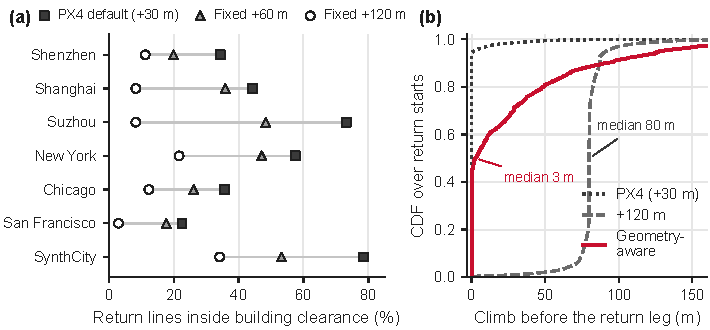
\includegraphics[width=\textwidth]{figures/pdf/m1_return_geometry.pdf}
\caption{F1, return geometry. (a) Share of straight return lines that enter the building clearance envelope for
three fixed return altitudes, drone at 40\,m above ground, 50,000 return starts per city. (b) Climb before the return leg over the six real
cities: fixed altitudes climb for every return; a geometry-aware altitude climbs only where the line requires it}
\label{fig:m1}
\end{figure}

\paragraph{F2: Wind breaks decisions through feasibility and model disagreement.}
We fly 800\,m legs on eight headings in the synthetic city under a reference-wind sweep from 0 to 16\,m/s
(Fig.~\ref{fig:m2}). Two observations stand out. First, the energy drawn per second barely changes with wind in our
reference model: below 10\,m/s the change is within $\pm$1\%, as expected on the flat bottom of the U-shaped
power curve of multirotors, where the induced power saved at higher airspeed offsets the added parasitic
power~\cite{liu2017power,bauersfeld2022range}; and a wind-blind estimate of the flown trajectory stays
within 2.5\% of the energy actually drawn (Fig.~\ref{fig:m2}b). Wind costs energy mainly through the longer
flight time against a headwind, which the shared model captures. What wind does change is \emph{feasibility}: beyond the
vehicle's 13.8\,m/s rating no leg completes. Second, and more surprisingly, wind exposes \emph{model disagreement}
between modules. When the return trigger uses its own time-based headwind model (ground speed reduced by the
headwind), as a stand-alone failsafe does, it predicts a return that the planner's energy model considers easy, and it
aborts 15--25\% of feasible legs between 2 and 12\,m/s (Fig.~\ref{fig:m2}a). When the trigger evaluates the same energy
model as the precheck, every leg below 10\,m/s completes. Wind-aware decisions thus need one shared energy and wind
model, not a better estimator in one module.

\begin{figure}[t]
\centering
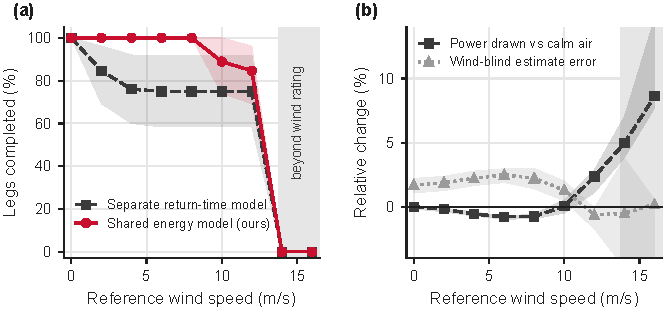
\includegraphics[width=\textwidth]{figures/pdf/m2_wind_feasibility.pdf}
\caption{F2, wind. Closed-loop 800\,m outbound and return legs, 3 seeds and 6 headings per wind speed; shaded bands are 95\%
bootstrap intervals; the shaded region on the right lies beyond the vehicle's 13.8\,m/s wind rating. (a) Legs completed when the return trigger uses a separate time-based headwind model vs the
planner's shared energy model. (b) Electrical power drawn relative to calm air, and the error of a wind-blind energy
estimate of the same trajectory}
\label{fig:m2}
\end{figure}

\paragraph{F3: A weather-blind scan plan misses targets and does not know it.}
We plan a recognition-level scan of a 500\,m area of interest at the altitude that meets the target ground sample
distance in clear air, place 400 human-sized targets on open ground, and evaluate each target's perception level with
the Johnson criteria~\cite{sjaardema2015history,vollmerhausen2004new}, using the line of sight to the camera and the
contrast attenuated by the environment field's optical depth~\cite{horvath1971koschmieder}. Figure~\ref{fig:m3}a
sweeps the meteorological optical range (MOR) for plans made for detection, recognition and identification. In clear
air about 90\% of targets reach the level; the rest are occluded by buildings. The share then collapses like a cliff,
not a slope: the recognition plan loses almost all targets between 500 and 300\,m MOR, and the detection and
identification plans, which fly at different heights, fall off between 300 and 200\,m. Across the presets
(Fig.~\ref{fig:m3}b), the weather-blind plan keeps its clear-air capture in rain, snow and thunderstorms, where
visibility stays above 0.8\,km, but the recognition plan captures 5\% of targets in fog, 0\% in a blizzard and 73\% in
a sandstorm (90\% in clear air), while predicting 99\% coverage in every case. The failure is silent: the plan is
geometrically complete, and nothing in it signals that the camera cannot see.

\begin{figure}[t]
\centering
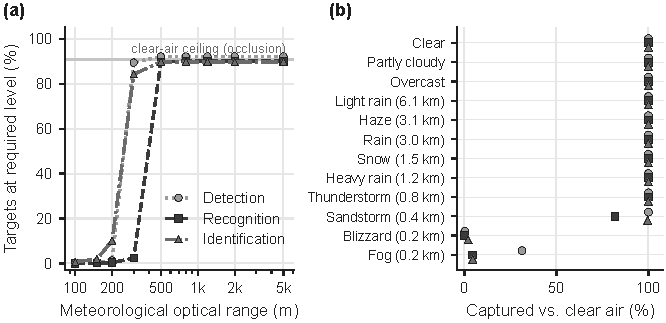
\includegraphics[width=\textwidth]{figures/pdf/m3_perception_gap.pdf}
\caption{F3, perception. (a) Targets that reach the required perception level under a scan plan made for clear air, as
the meteorological optical range (MOR) varies; 7 cities, 3 seeds per MOR. The ceiling is set by building occlusion.
(b) Capture of the same plan per weather preset relative to clear air, presets sorted by their MOR}
\label{fig:m3}
\end{figure}

\paragraph{F4: Naive coupling does not fit in the tick.}
Coupling multiplies queries: every return plan needs a corridor query along the line home, wind at the return
altitude and an energy integral, and it goes stale as the drone and the weather move. We time the naive way of keeping
every plan current, one process pinned to one core of a 64-core server (Fig.~\ref{fig:m4}). Refreshing every drone's
plan at every 4\,ms tick with an exact corridor query costs 53.8\,ms per refresh at 1,000 drones, or 13.4
core-seconds per simulated second: thirteen cores for one decision, 34 times the 0.40 core-seconds the whole pipeline
may use. Even with a sampled corridor the same schedule costs 0.15 core-seconds per simulated second, more than a third
of the pipeline budget for a single decision. Query granularity matters as much: one wind query per point costs
27.8\,$\mu$s, against 0.16\,$\mu$s per point in a batch of 10,000. Coupled decisions are therefore affordable only if
queries are batched and scheduled, not issued per drone and per tick.

\begin{figure}[t]
\centering
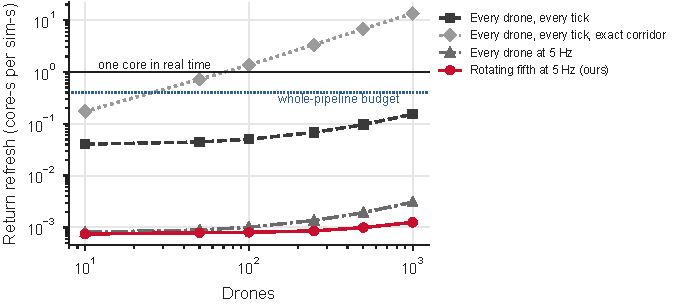
\includegraphics[width=0.86\textwidth]{figures/pdf/m4_coupling_cost.pdf}
\caption{F4, cost of coupling. CPU time to keep every drone's return plan current, per simulated second, on one core;
median of three runs. Exact corridor queries every tick exceed a full core beyond about 70 drones; the runtime's
rotating 5\,Hz schedule (Sect.~\ref{sec:design:runtime}) stays near one core-millisecond per simulated second}
\label{fig:m4}
\end{figure}


\subsection{Goals and challenges}\label{sec:bg:challenges}

The findings define three goals: decisions that see geometry, weather and energy together (F1--F3); one model shared by
the planner, the runtime and the display, so that modules do not contradict each other (F2); and coupled decisions for
a whole fleet in real time on hardware an operator actually has (F4). Reaching them raises five challenges.

\begin{description}
\item[C1 One queryable city.] City geometry arrives as point clouds, terrain models, building footprints and no-fly
zones, each with its own resolution and frame. Decisions need fast, exact answers (the highest roof along a line,
line of sight, clearance of a path) from one merged, versioned world.
\item[C2 One consistent model.] The planner, the runtime and the display must evaluate the same wind, visibility and
energy at the same place and time. Otherwise a precheck accepts what the failsafe aborts (F2) or the display shows
weather the decision did not use.
\item[C3 Perception under occlusion and weather.] Whether a target is seen depends on resolution, line of sight and
atmospheric contrast; a scan planner must work backwards from a required perception level to a flight height and
must account for visibility.
\item[C4 Real time for a fleet.] Coupled queries must fit into the 4\,ms simulation tick for 1,000 drones on a
CPU-only server.
\item[C5 Access without a server GPU.] Operators watch and steer the fleet from ordinary browsers and laptops; the
server must not render, and the client must stream a city-scale point cloud within its own budget.
\end{description}

\subsection{Related work}\label{sec:bg:related}

\paragraph{Drone simulators.} AirSim and Cosys-AirSim~\cite{shah2017airsim,jansen2023cosysairsim} render photorealistic
Unreal scenes; their wind is a single world-frame vector and their weather is a set of visual effects. Gazebo with PX4
software-in-the-loop (SITL) simulation~\cite{koenig2004gazebo,meier2015px4,furrer2016rotors} offers a uniform wind model with gusts and a linear battery
drain that feeds the failsafes. Flightmare~\cite{song2020flightmare}, gym-pybullet-drones~\cite{panerati2021learning},
RotorPy~\cite{folk2023rotorpy} and Crazyflow~\cite{schuck2026crazyflow} target control and learning; RotorPy and
Crazyflow batch more than 1,000 drones on a CPU but have no city geometry. OmniDrones~\cite{xu2024omnidrones}, Aerial
Gym~\cite{kulkarni2025aerialgym} and Pegasus~\cite{jacinto2024pegasus} build on NVIDIA Isaac
Sim~\cite{nvidia2025isaaclab,mittal2023orbit} and need a GPU. Swarm platforms such as
ARGoS~\cite{pinciroli2012argos}, SwarmLab~\cite{soria2020swarmlab}, XTDrone~\cite{xiao2020xtdrone} and the MRS
system~\cite{baca2021mrs} focus on coordination and deployment rather than on the city and the weather. CARLA, the
reference simulator for urban driving, states that weather does not affect physics~\cite{dosovitskiy2017carla}.

\paragraph{City models and aerial agents.} Embodied aerial benchmarks place agents in city scenes:
AerialVLN~\cite{liu2023aerialvln}, CityNav~\cite{lee2025citynav}, EmbodiedCity~\cite{gao2024embodiedcity} and
OpenFly~\cite{gao2025openfly}, and AerialClaw~\cite{li2026aerialclaw} drives aerial agents with language models.
Their cities are modelled for vision, and weather, energy and fleet scale are outside their scope. Urban digital
twins~\cite{batty2018digitaltwins,ketzler2020digitaltwins,shahat2021citydigitaltwin} and Web 3D formats and viewers
(3D Tiles, Potree)~\cite{ogc2023_3dtiles,schuetz2020octree,discher2019webpointclouds} stream real geometry to browsers
but do not simulate vehicles.

\paragraph{Energy, wind and return.} Multirotor power models~\cite{liu2017power,stolaroff2018energy,dorling2017vehicle,zhang2021energy}
and range estimation~\cite{bauersfeld2022range} underpin energy-aware planning; wind-aware routing for delivery
drones~\cite{ito2022wind,chakrabarty2011energy} and emergency planning under energy limits~\cite{tenharmsel2017emergency}
show that wind and energy change the best route. Studies of the urban wind
field~\cite{galway2011urban,ware2016analysis,kakavitsas2024quadrotor} and of global flyability~\cite{gao2021weather}
show how strongly the city shapes the wind and how often weather grounds drones. These works optimise one decision
under one model; we provide the shared model that lets the precheck, the return trigger and the display agree.

\paragraph{Coverage and perception.} Coverage path planning is well
surveyed~\cite{galceran2013survey,cabreira2019survey}; boustrophedon decompositions~\cite{choset2000coverage,coombes2017boustrophedon}
and energy-aware coverage~\cite{difranco2016coverage} fix the strip spacing from the camera footprint. The Johnson
criteria and the targeting task performance metric~\cite{sjaardema2015history,vollmerhausen2004new} predict the
probability of detecting, recognising and identifying a target from its resolved size and contrast, and Koschmieder's
law~\cite{horvath1971koschmieder} links contrast to visibility. We connect them: the scan planner works backwards from
the required perception level, through the visibility of the 4D field, to the flight height, strip spacing and fleet
size. Task allocation uses the contract net protocol~\cite{smith1980contract}, market-based
coordination~\cite{dias2006market,choi2009consensus} and the Hungarian method~\cite{kuhn1955hungarian}.

\paragraph{Comparison.} Table~\ref{tab:related} compares representative systems on the capabilities that coupled
urban decisions need. No existing system combines real city geometry at city scale, a weather field that drives both
the dynamics and the sensing, energy-aware decisions and 1,000-drone scale on a CPU-only server with browser access.

\begin{table}[t]
\caption{Capabilities needed for coupled urban drone decisions. \yes{} supported, \prt{} partial or only through
user-supplied assets, \no{} not supported or not documented. Evidence for every cell (documentation pages, papers) is
listed in the supplementary material.}
\label{tab:related}
\scriptsize
\setlength{\tabcolsep}{4pt}
\newcommand{\rot}[1]{\rotatebox{90}{\parbox{1.9cm}{\raggedright #1}}}
\begin{tabular*}{\textwidth}{@{\extracolsep\fill}lcccccccccc@{}}
\toprule
 & \multicolumn{2}{c}{Geometry} & \multicolumn{2}{c}{Weather} & & & \multicolumn{2}{c}{Access} & & \\
\cmidrule(lr){2-3}\cmidrule(lr){4-5}\cmidrule(lr){8-9}
System & \rot{Real city} & \rot{City scale} & \rot{Drives dynamics} & \rot{Affects sensing} & \rot{Energy-aware decisions}
 & \rot{$\geq$1,000 drones} & \rot{No server GPU} & \rot{Browser} & \rot{Deterministic replay} & \rot{Open source} \\
\midrule
AirSim/Cosys-AirSim~\cite{shah2017airsim,jansen2023cosysairsim} & \prt & \prt & \prt & \prt & \no & \no & \no & \no & \no & \yes \\
Gazebo+PX4 SITL~\cite{koenig2004gazebo,meier2015px4} & \prt & \prt & \prt & \no & \prt & \no & \prt & \prt & \prt & \yes \\
Flightmare~\cite{song2020flightmare} & \no & \no & \no & \no & \no & \prt & \prt & \no & \no & \yes \\
gym-pybullet-drones~\cite{panerati2021learning} & \no & \no & \no & \no & \no & \no & \yes & \no & \no & \yes \\
RotorPy~\cite{folk2023rotorpy} & \no & \no & \prt & \no & \no & \yes & \yes & \no & \no & \yes \\
Crazyflow~\cite{schuck2026crazyflow} & \no & \no & \no & \no & \no & \yes & \yes & \no & \no & \yes \\
OmniDrones~\cite{xu2024omnidrones} & \no & \no & \no & \no & \no & \prt & \no & \no & \no & \yes \\
Aerial Gym~\cite{kulkarni2025aerialgym} & \no & \no & \no & \no & \no & \yes & \no & \no & \no & \yes \\
Pegasus~\cite{jacinto2024pegasus} & \no & \no & \no & \no & \no & \no & \no & \no & \no & \yes \\
Isaac Sim/Lab~\cite{nvidia2025isaaclab,mittal2023orbit} & \no & \no & \no & \no & \no & \prt & \no & \prt & \no & \prt \\
MRS UAV System~\cite{baca2021mrs} & \no & \no & \no & \no & \no & \no & \no & \no & \no & \yes \\
CARLA (driving)~\cite{dosovitskiy2017carla} & \no & \prt & \no & \prt & \no & \no & \prt & \no & \yes & \yes \\
OpenFly~\cite{gao2025openfly} & \prt & \yes & \no & \no & \no & \no & \no & \no & \no & \yes \\
EmbodiedCity~\cite{gao2024embodiedcity} & \prt & \yes & \no & \no & \no & \no & \no & \prt & \no & \prt \\
CesiumJS/3D Tiles~\cite{ogc2023_3dtiles} & \yes & \yes & \no & \no & \no & \no & \yes & \yes & \no & \yes \\
Potree~\cite{schuetz2020octree} & \yes & \yes & \no & \no & \no & \no & \yes & \yes & \no & \yes \\
\midrule
\textbf{This work} & \yes & \yes & \yes & \yes & \yes & \yes & \yes & \yes & \yes & \yes \\
\botrule
\end{tabular*}
\end{table}

